
\documentclass[usenames,dvipsnames]{beamer}
\usepackage[utf8]{inputenc}
\usepackage{stmaryrd}
\usepackage{verbatim}

\usetheme{Padova}




\usepackage[utf8]{inputenc}
\usepackage{graphics}
\usepackage[T1]{fontenc}
\usepackage{lmodern}
\usepackage{mathpartir}
\usepackage{mathrsfs}
\usepackage[all]{xy}
\usepackage{amsfonts}



\usepackage[mathscr]{eucal}
\usepackage{ragged2e}
\addtobeamertemplate{theorem begin}{}{\justifying}
\addtobeamertemplate{block begin}{}{\justifying}
\addtobeamertemplate{exampleblock begin}{}{\justifying}
\addtobeamertemplate{alertblock begin}{}{\justifying}
%%% Bibliography
\usepackage[style=authoryear,backend=bibtex]{biblatex}
\addbibresource{bibliog.bib}


\newcommand{\terms}[1]{\mathcal{{#1}}\text{-}\mathsf{Terms}}
\makeatletter
\renewcommand{\itemize}[1][]{%
	\beamer@ifempty{#1}{}{\def\beamer@defaultospec{#1}}%
	\ifnum \@itemdepth >2\relax\@toodeep\else
	\advance\@itemdepth\@ne
	\beamer@computepref\@itemdepth% sets \beameritemnestingprefix
	\usebeamerfont{itemize/enumerate \beameritemnestingprefix body}%
	\usebeamercolor[fg]{itemize/enumerate \beameritemnestingprefix body}%
	\usebeamertemplate{itemize/enumerate \beameritemnestingprefix body begin}%
	\list
	{\usebeamertemplate{itemize \beameritemnestingprefix item}}
	{\def\makelabel##1{%
			{%
				\hss\llap{{%
						\usebeamerfont*{itemize \beameritemnestingprefix item}%
						\usebeamercolor[fg]{itemize \beameritemnestingprefix item}##1}}%
			}%
		}%
	}
	\fi%
	\beamer@cramped%
	\justifying% NEW
	%\raggedright% ORIGINAL
	\beamer@firstlineitemizeunskip%
}
\makeatother


% Author names in publication list are consistent 
% i.e. name1 surname1, name2 surname2
% See https://tex.stackexchange.com/questions/106914/biblatex-does-not-reverse-the-first-and-last-names-of-the-second-author
%\DeclareNameAlias{author}{first-last}

%%% Suppress biblatex annoying warning
\usepackage{silence}
\WarningFilter{biblatex}{Patching footnotes failed}
\usepackage{physics}
%%% Some useful commands
% pdf-friendly newline in links
\newcommand{\pdfnewline}{\texorpdfstring{\newline}{ }} 
% Fill the vertical space in a slide (to put text at the bottom)


% direct shift
\newcommand{\shift}[1]{\ensuremath{\mathrel{{\leftrightsquigarrow}_{#1}}}}

% shift equivalence
\newcommand{\shifteq}[1][]{\ensuremath{\mathrel{{\equiv}^\mathit{sh}_{#1}}}}

\newcommand{\dder}[1]{\mathscr{#1}}
\usepackage{ragged2e}
\addtobeamertemplate{theorem begin}{}{\justifying}
\addtobeamertemplate{block begin}{}{\justifying}
\addtobeamertemplate{exampleblock begin}{}{\justifying}
\addtobeamertemplate{alertblock begin}{}{\justifying}
\addtobeamertemplate{block alerted begin}{}{\justifying}

\usepackage{etoolbox}
\apptocmd{\thebibliography}{\justifying}{}{} 

\usepackage{mathpartir}
\usepackage[usestackEOL]{stackengine}
\usepackage{mathtools,amssymb}
%\newcommand{\ar}[0]{\mathsf{ar}}
\newcommand{\comma}[2]{#1\hspace{1pt} {\downarrow}\hspace{1pt} #2}
\newcommand{\ex}[2]{\mathsf{m}\qty(#1, #2)}
\newcommand{\ext}[2]{\mathsf{m}\qty(#1, #2)}
\newcommand{\cri}[1]{\mathsf{cri}\hspace{-.4pt}\left({#1}\right)}
\newcommand\functorop[1][l]{\csname#1functor\endcsname}
\newcommand\lfunctorop[3]{%
	\setbox0=\hbox{$#2$}%
	\kern\wd0%
	\ensurestackMath{\Centerstack[c]{#1\\ \mathllap{#2\;\,}\mathclap{\DownArrow}\\#3}}%
}
\newcommand\rfunctorop[3]{%
	\setbox0=\hbox{$#2$}%
	\ensurestackMath{\Centerstack[c]{#1\\\mathclap{\UpArrow}\mathrlap{\,\;#2}\\#3}}%
	\kern\wd0%
}
\newcommand\functoropmapsto{\mathrel{\ensurestackMath{\Centerstack[c]{\longmapsto\\ \\\longmapsto}}}}
\setstackgap{L}{1.3\normalbaselineskip}
\newcommand\UpArrow{\rotatebox[origin=c]{90}{$\longrightarrow$\,}}
\newcommand\DownArrow{\rotatebox[origin=c]{-90}{$\longrightarrow$\,}}

\newcommand{\arro}[0]{\mathrel{\rotatebox[origin=c]{270}{$\twoheadrightarrow$}}}

\newcommand{\arr}[2]{{#1}{\arro}{\catname{#2}}}
\newcommand\functor[1][l]{\csname#1functor\endcsname}

\newcommand{\tg}[0]{\catname{TG}_{\Sigma}}
\newcommand{\ari}[0]{\mathsf{ar}}
\newcommand{\lgt}[0]{\mathsf{length}}

\newcommand{\cma}[2]{\mathcal{#1}\hspace{1pt} {\downarrow}\hspace{1pt} \mathcal{#2}}
\newcommand\lfunctor[3]{%
	\setbox0=\hbox{$#2$}%
	\kern\wd0%
	\ensurestackMath{\Centerstack[c]{#1\\ \mathllap{#2\;\,}\mathclap{\DownArrow}\\#3}}%
}
\newcommand\rfunctor[3]{%
	\setbox0=\hbox{$#2$}%
	\ensurestackMath{\Centerstack[c]{#1\\\mathclap{\DownArrow}\mathrlap{\,\;#2}\\#3}}%
	\kern\wd0%
}
\newcommand\functormapsto{\mathrel{\ensurestackMath{\Centerstack[c]{\longmapsto\\ \\\longmapsto}}}}
\setstackgap{L}{1.3\normalbaselineskip}
%\newcommand\DownArrow{\rotatebox[origin=c]{-90}{$\longrightarrow$\,}}


\newcommand{\framefill}{\vskip0pt plus 1filll}
\newcommand{\vin}{\rotatebox[origin=c]{-90}{$\dashv$}}
\newcommand{\catname}[1]{{\normalfont\textbf{#1}}}
\newcommand{\homodd}[0]{\catname{HoMod}}
\newcommand{\jp}[0]{\mathfrak{j}_{\mathcal{M}, \mathcal{N}}}
\newcommand{\slice}[2]{(\catname{#1}\downarrow{#2})}
\newcommand{\supp}[1]{\mathsf{supp}({#1},\mu_{#1})}
%\newcommand{\norm}[1]{\left\lVert#1\right\rVert}
%\newcommand{\abs}[1]{\left\lvert#1\right\rvert}
\newcommand{\nat}{\mathsf{nat}}
\newcommand{\y}{\mathsf{y}}
\newcommand{\im}[1]{\mathrm{Im}(#1)}
\newcommand{\chain}[1]{\catname{Ch}(\catname{#1})}
\newcommand{\homo}[1]{\mathcal{K}(\catname{#1})}
\newcommand{\colim}[0]{\mathrm{colim}}
\newcommand{\rela}[2]{\mathscr{Rel}_\mathcal{#2}(\catname{#1})}
\newcommand{\sub}{\mathsf{Sub}}
\newcommand{\dom}{\mathrm{dom}}
\newcommand{\cod}{\mathrm{cod}}
\newcommand{\co}[1]{\{\abs{#1}\}}
\newcommand{\eq}[3]{[#1 = #2]_{#3}}
\newcommand{\equ}[2]{[#1 \equiv #2]}
\newcommand{\rel}[3]{\frak{R}_{\mathcal{#3}}(#1, #2)}
\newcommand{\sat}[0]{\mathsf{cl}}
\newcommand{\cov}{\vartriangleleft}
\newcommand{\pos}[1]{\mathsf{Pos}_{\mathfrak{#1}}}
\newcommand{\rk}[2]{\mathrm{rk}_{#1}({#2})}
\newcommand{\lind}[1]{\mathcal{L}({#1})}
\newcommand{\class}[1]{\catname{Cl}({#1})}
\newcommand{\hoclass}[1]{\catname{HoCl}({#1})}
\newcommand{\propo}[0]{\mathsf{Prop}}
\newcommand{\term}[2]{\mathbf{Term}({#1}, {#2})}
\newcommand{\formu}[1]{\mathbf{Form}_{#1}}
%\newcommand{\ex}[1]{\mathscr{ex(#1)}}
\newcommand{\inte}[1]{\llbracket{#1}\rrbracket}
\newcommand{\typ}[1]{\mathsf{Type}({#1})}
\newcommand{\Set}{\textbf{\textup{Set}}}
\newcommand{\m}[1]{\textbf{\textup{#1}}}
\newcommand{\sh}{\textbf{\textup{Sh}}}
\NewDocumentCommand{\transp}{m o}{%
	\ensuremath{({#1},%
		\IfNoValueTF{#2}%
		{{#1}+1}%
		{#2}%
		)}
}

\newcommand{\inv}[1]{\mathsf{inv}({#1})}





\newcommand{\modd}[0]{\catname{Mod}}
\newcommand{\des}[1]{Des({#1})}
\newcommand{\prof}[2]{\mathsf{Proof}({#1},{#2})}
\newcommand{\ab}[0]{=-Adj}
\newcommand{\ba}[0]{=-E}
\newcommand{\su}[2]{\mathfrak{s}_{#1}^{#2}}
\newcommand{\ipos}[1]{\catname{Pos}(\catname{#1})}
\newcommand{\Su}[2]{\mathfrak{S}_{#1}^{#2}}
\newcommand{\Pro}[2]{\mathfrak{P}_{#1}^{#2}}
\newcommand{\surr}[0]{\mathsf{surr}}
\newcommand{\propag}[0]{\mathsf{propag}}
\newcommand{\mdl}[1]{\catname{Mod}(#1)}
\newcommand{\alg}[1]{\catname{FAlg}(#1)}
\newcommand{\eim}[1]{\catname{EM}(\m{#1})}
\def\H{\textbf {\textup{H}}}
\def\X{\textbf {\textup{X}}}
\def\Y{\textbf {\textup{Y}}}
\newcommand{\fuz}[1]{\textbf{\textup{Fuz}}({\textbf {\textup{#1}}})}
%\newcommand{\yo}{\mathcal{Y}}
\renewcommand*{\bibfont}{\footnotesize}

\newcommand{\der}[1]{\underline{\dder{#1}}}


\DeclareFontFamily{U}{dmjhira}{}
\DeclareFontShape{U}{dmjhira}{m}{n}{
	<-> s*[0.95] dmjhira
}{}
\DeclareFontSubstitution{U}{dmjhira}{m}{n}

\newcommand{\yo}{%
	\raisebox{0.2\depth}[\fontcharht\font`A][0.1\depth]{%
		\usefont{U}{dmjhira}{m}{n}\symbol{"48}%
	}%
}

\usepackage{tikz-cd}
\usepackage{tikz}
\usetikzlibrary{arrows,shapes,snakes,automata,backgrounds,petri,fit,positioning,calc}
\tikzstyle{node}=[circle, draw=black, minimum size=1mm, inner sep=1.5pt, font=\tiny]

\tikzstyle{trans}=[font=\scriptsize]
\tikzstyle{lab}=[font=\small]
\tikzset{
	coloredge/.style={
		->,
		color=red
		%densely dotted
	}
}

\tikzset{
	colorloop/.style={
		loop,
		color=red
		%densely dotted
	}
}

\tikzcdset{
	perm/.style={
		shorten >=-1mm, shorten <=-1mm,
		-,
		% dotted
	}
}


\newcommand{\pgfBox}{
	\begin{pgfonlayer}{background} 
		\fill[blue!2,thick,draw=black!50,rounded corners,inner sep=3mm] ([xshift=-1.5pt,yshift=-1.5pt]current bounding box.south west) rectangle ([xshift=1.5pt,yshift=1.5pt]current bounding box.north east);
	\end{pgfonlayer}
}


\newcommand{\id}[1]{\mathsf{id}_{#1}}

\title{Left-Linear Rewriting in Adhesive Categories}

\date[May 1977]{Calgary, September 11, 2024}
\begin{document}
	\maketitle 


\begin{frame}{Concurrency}\justifying
	

	
	Key  idea of concurrency theory:  the behaviour of a computational
	device can be modelled by abstracting its sequences of steps via a suitable equivalence.
	
	\pause 
	\medskip 
	The equivalence captures when steps are causally unrelated and thus could be
	executed in \emph{any} order, and possibly in \emph{parallel}.
	
	\pause 
	\medskip 
	Defining this equivalence often boils down to having a notion
	of \emph{independence} between two consecutive steps. 
	
	
\end{frame}


\begin{frame}{DPO rewriting sytems}\justifying
	
	
		We will focus on the \emph{double pushout} (DPO) approach  to  graph rewriting (cfr. \cite{ehrig2006fundamentals}).
	
	\smallskip 
	\begin{overprint}
		\onslide<1|handout:1>
		A \emph{rewriting rule} is a pair  of arrows $l:K\to L$ and $r:K\to R$ with the same domain. To rewrite an object $G$ according to a rule we proceed in three steps.
		
		\onslide<2| handout:0>
		
		A \emph{rewriting rule} is a pair  of arrows $l:K\to L$ and $r:K\to R$ with the same domain. To rewrite an object $G$ according to a rule we proceed in three steps.
		
		First: find a \emph{match} $m:L\to G$.
		\begin{center}
			\begin{tikzpicture}
				\node(L)at(0,0){$L$};
				\node(K)at(2,0){$K$};
				\node(R)at(4,0){$R$};
				\node(G)at(0,-2){$G$};
				\draw[->](K)--(L)node[pos=0.5, above]{$l$};
				\draw[->](K)--(R)node[pos=0.5, above]{$r$};
				\draw[->, dotted](L)--(G)node[pos=0.5, left]{$m$};
			\end{tikzpicture}
		\end{center}
		
		
		\onslide<3| handout:0>

A \emph{rewriting rule} is a pair  of arrows $l:K\to L$ and $r:K\to R$ with the same domain. To rewrite an object $G$ according to a rule we proceed in three steps.		
		
		Second: remove the image of $m$  building a pushout square. \vspace{-0.075cm}
		\begin{center}
			\begin{tikzpicture}
				\node(L)at(0,0){$L$};
				\node(K)at(2,0){$K$};
				\node(R)at(4,0){$R$};
				\node(G)at(0,-2){$G$};
				\node(C)at(2,-2){$C$};
				\draw[->](K)--(L)node[pos=0.5, above]{$l$};
				\draw[->](K)--(R)node[pos=0.5, above]{$r$};
				\draw[->](L)--(G)node[pos=0.5, left]{$m$};
				\draw[->, dotted](K)--(C)node[pos=0.5, right]{$p$};
				\draw[->, dotted](C)--(G)node[pos=0.5, below]{$l'$};
			\end{tikzpicture}
		\end{center}		
		\onslide<4| handout:0>
		
		A \emph{rewriting rule} in a category $\X$ is a pair  of arrows $l:K\to L$ and $r:K\to R$ with the same domain. To rewrite an object $G$ according to a rule we proceed in three steps.
		
		Third: fill the hole so obtained, with $R$ taking a pushout.\vspace{-0.075cm}
		\begin{center}\hspace{0.045cm}
			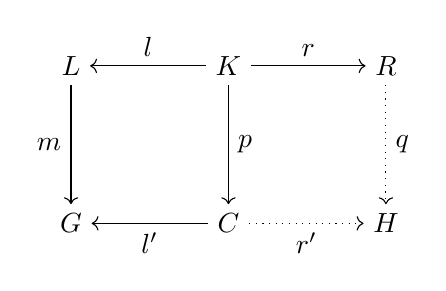
\begin{tikzpicture}
				\node(L)at(0,0){$L$};
				\node(K)at(2,0){$K$};
				\node(R)at(4,0){$R$};
				\node(G)at(0,-2){$G$};
				\node(C)at(2,-2){$C$};
				\node(H)at(4,-2){$H$};
				\draw[->](K)--(L)node[pos=0.5, above]{$l$};
				\draw[->](K)--(R)node[pos=0.5, above]{$r$};
				\draw[->](L)--(G)node[pos=0.5, left]{$m$};
				\draw[->](K)--(C)node[pos=0.5, right]{$p$};
				\draw[->](C)--(G)node[pos=0.5, below]{$l'$};
				\draw[->, dotted ](C)--(H)node[pos=0.5, below]{$r'$};
				\draw[->, dotted ](R)--(H)node[pos=0.5, right]{$q$};
			\end{tikzpicture}
		\end{center}		
	\end{overprint}  	
\end{frame}

\begin{frame}{DPO rewriting system}\justifying
The categorical framework is given by \emph{$\mathcal{M}$-adhesive categories}. \pause 
\begin{definition}[\cite{lack2005adhesive,azzi2019essence,ehrig2014adhesive}]
	Let $\mathcal{M}$ be a class of monos in a category $\X$, containing all isomorphisms, stable under pullbacks and composition. $\X$ is \emph{$\mathcal{M}$-adhesive} if, given a cube below with the hooked arrows in $\mathcal{M}$, the bottom face a pushout and the back faces pullbacks, we have:
	
	\parbox{5cm}{\centering 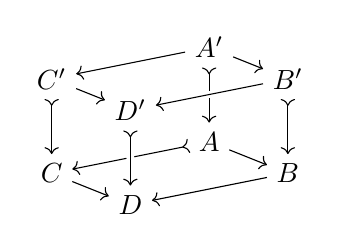
\begin{tikzpicture}
		\node(C)at(-1,0.4){$C$};
		\node(A)at(1,0.8){$A$};
		\node(B)at(2,0.4){$B$};
		\node(D)at(0,0){$D$};
		\node(A')at(1,2){$A'$};
		\node(B')at(2,1.6){$B'$};
		\node(C')at(-1,1.6){$C'$};
		\node(D')at(0,1.2){$D'$};
		\draw[<-](B')--(A');
		\draw[>->](B')--(B);
		\draw[>->](C')--(C); 
		\draw[>->](D')--(D);
		\draw[->](A')--(C'); 
		\draw[->](B')--(D');
		\draw[->](C')--(D');
		\draw[->](A)--(B);
		\draw[->](C)--(D);
		\draw[->](B)--(D);
		\draw[>-](A')--(1,1.45);
		\draw[->](1,1.35)--(A);
		\draw[>-](A)--(0.05, 0.61);
		\draw[<-](C)--(-0.05,0.59);
\end{tikzpicture}} \quad 	\parbox{4cm}{\centering
	Top face is a pushout \\ $\iff$ \\ Front faces are pullbacks}
	
\end{definition}
\end{frame}


\begin{frame}{DPO rewriting systems}\justifying
		\begin{definition}
		A \emph{DPO-rewriting system} is a pair $(\X, R)$ where $\X$ is an $\mathcal{M}$-adhesive category and $R$ is a set of rewriting rules.
		\pause 
		
		A system is \emph{linear} if every rule is made by arrows in $\mathcal{M}$, \emph{left-linear} if the left hand side of every rule is in $\mathcal{M}$.
	\end{definition}

\pause 

In left-linear rewriting systems a rule can ``merge'' parts of the state.

\pause 
\begin{alertblock}{Motivation}
	Our long term aim is to provide a concurrent semantics for left-linear DPO-rewriting systems (see \cite{baldan2017domains}). 
\end{alertblock}

\end{frame}


\begin{frame}{An example}\justifying
	
	We want to model a situation in which a coffee comes
	with a bag of white sugar and a bag of brown sugar.
	
	\pause 
\begin{figure}
	\begin{center}

  %%% RULES 
  % 
  % RULE add white sugar
  % 
  \begin{tikzpicture}[node distance=3mm, font=\small]
    %, baseline=(current bounding box.center), font=\small]
      \node (l) {
      \begin{tikzpicture}[node distance=2mm, label distance=1mm, font=\scriptsize]
      % 
      \node at (0,1.0) [node, label=left:$1$] (1) {}
        edge [in=110, out=140, loop] node[above] {$\mathit{m}$} ();

        \node at (0,0.6) {};

        \node at (0.7,1.0) [node, label=right:$2$] (2) {};

        \draw[->] (1) to node[above, pos=0.4]{$\mathit{s}$} (2);        
      %
      \pgfBox
      \end{tikzpicture} 
    };
    \node [right=of l] (r) {
      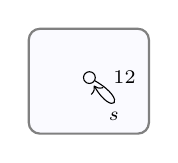
\begin{tikzpicture}[node distance=2mm, label distance=1mm, font=\scriptsize]
        %
        \node at (0,1.45) {};
        \node at (0,0.5) {};
        \node at (0.6,1.0) [node, label=right:$12$] (12) {}
          edge [in=300, out=330, loop] node[below] {$\mathit{s}$} (); 
      %
      \pgfBox
      \end{tikzpicture}
    };
    %\node[below] at (l.south east) {$\rho_w$};
    \path (l) edge[->] (r);
    \node at ($(l)!0.54!(r)$) [below=7.5mm] {$\rho_m$: add milk and sugar}; 
    \end{tikzpicture}
    % 
    %
    \hspace{5mm}
    % \hfill
    % 
    % RULE cocoa
    %
    \begin{tikzpicture}[node distance=3mm, font=\small]
    %, baseline=(current bounding box.center), font=\small]
      \node (l) {
      \begin{tikzpicture}[node distance=2mm, label distance=1mm, font=\scriptsize]
      % 
       \node at (0,1.0) [node, label=left:$1$] (1) {}
        edge [in=220, out=250, loop] node[below] {$\mathit{c}$} ();

        \node at (0,0.6) {};

        \node at (0.7,1.0) [node, label=right:$2$] (2) {};

        \draw[->] (1) to node[above, pos=0.4]{$\mathit{s}$} (2);
        
      %
      \pgfBox
      \end{tikzpicture} 
    };
    \node [right=of l] (r) {
      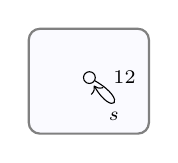
\begin{tikzpicture}[node distance=2mm, label distance=1mm, font=\scriptsize]
      %
      \node at (0,1.45) {};  
      \node at (0,0.5) {};
      \node at (0.6,1.0) [node, label=right:$12$] (12) {}
          edge [in=300, out=330, loop] node[below] {$\mathit{s}$} ();        
      %
      \pgfBox
      \end{tikzpicture}
    };
    \path (l) edge[->]  (r);
    \node at ($(l)!0.54!(r)$) [below=7.5mm] {$\rho_c$: add cocoa and sugar};         
    \end{tikzpicture}
    %
    \hspace{5mm}
    % RULE ready
    % 
    \begin{tikzpicture}[node distance=3mm, font=\small]
    %, baseline=(current bounding box.center), font=\small]
      \node (l) {
      \begin{tikzpicture}[node distance=2mm, label distance=1mm, font=\scriptsize]
      % 
      \node at (0.4,0.5) {};
      \node at (0.6,1.0) [node, label=right:$1$] (1) {}
        edge [in=40, out=70, loop] node[above] {$\mathit{u}$} ()
        edge [in=300, out=330, loop] node[below] {$\mathit{s}$} ();
      %
      \pgfBox
      \end{tikzpicture} 
    };
    \node [right=of l] (r) {
      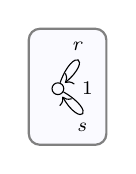
\begin{tikzpicture}[node distance=2mm, label distance=1mm, font=\scriptsize]
      % 
      \node at (0.4,0.5) {};
      \node at (0.6,1.0) [node, label=right:$1$] (1) {}
        edge [in=40, out=70, loop] node[above] {$\mathit{r}$} ()
        edge [in=300, out=330, loop] node[below] {$\mathit{s}$} ();
      %
      \pgfBox
      \end{tikzpicture}
    };
    \path (l) edge[->] (r);    
    \node at ($(l)!0.54!(r)$) [below=7.5mm] {$\rho_s$: stir and drink!}; 
    \end{tikzpicture}
  %
\end{center}

%%% Local Variables:
%%% mode: latex
%%% TeX-master: "../final"
%%% End:


\end{figure}
\end{frame} 

\begin{frame}{An example}
	If we want a (very sweet) coffee we can add first the white sugar and then the brown one. Finally we can stir it.
	\pause 
\begin{figure}
	\begin{center}

  %%% REWRITING 
  % 
  %
  % 
  \begin{tikzpicture}[node distance=8mm, font=\small]
    % graph G0
    \node (G0) {
      \begin{tikzpicture}[node distance=2mm, label distance=1mm, font=\scriptsize]
        % 
        \node at (0,1.0) [node, label=left:$1$] (1) {}
        edge [in=110, out=140, loop] node[above] {$\mathit{m}$} ()
        edge [in=220, out=250, loop] node[below] {$\mathit{c}$} ();
        
        \node at (0.7,1.0) [node, label=right:$2$] (2) {}
        edge [in=40, out=70, loop] node[above] {$\mathit{u}$} ();

        \draw[->] (1) to node[above, pos=0.4]{$s$} (2);        
      %
      \pgfBox
      \end{tikzpicture} 
    };
    \node[below] at (G0.south) {$G_0$};
    % graph G1
    \node [right=of G0] (G1) {
      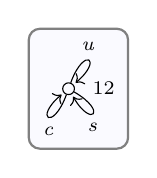
\begin{tikzpicture}[node distance=2mm, label distance=1mm,, font=\scriptsize]
      % 
      \node at (0.6,1.0) [node, label=right:$12$] (12) {}
        edge [in=220, out=250, loop] node[below] {$\mathit{c}$} ()
        edge [in=40, out=70, loop] node[above] {$\mathit{u}$} ()
        edge [in=300, out=330, loop] node[below] {$\mathit{s}$} ();        
      %
      \pgfBox
      \end{tikzpicture}
    };
    \node[below] at (G1.south) {$G_1$};

    % graph G2
    \node [right=of G1] (G2) {        
      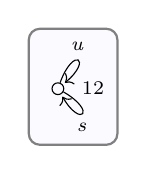
\begin{tikzpicture}[node distance=2mm, label distance=1mm, font=\scriptsize]
        %
        \node at (0.4,0.5) {};
      \node at (0.6,1.0) [node, label=right:$12$] (12) {}
%        edge [in=220, out=250, loop] node[below] {$\mathit{b}$} ()
        edge [in=40, out=70, loop] node[above] {$\mathit{u}$} ()
        edge [in=300, out=330, loop] node[below] {$\mathit{s}$} ();        
      %
      \pgfBox
    \end{tikzpicture}
    };
    \node[below] at (G2.south) {$G_2$};

    % graph G3
    \node [right=of G2] (G3) {      
      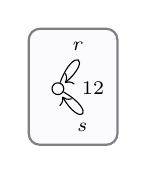
\begin{tikzpicture}[node distance=2mm, label distance=1mm, font=\scriptsize]
        %
        \node at (0.4,0.5) {};
      \node at (0.6,1.0) [node, label=right:$12$] (12) {}
%        edge [in=220, out=250, loop] node[below] {$\mathit{b}$} ()
        edge [in=40, out=70, loop] node[above] {$\mathit{r}$} ()
        edge [in=300, out=330, loop] node[below] {$\mathit{s}$} ();        
        % 
        \pgfBox
      \end{tikzpicture}
    };
    \node[below] at (G3.south) {$G_3$};
   
    \path (G0) edge[->] node[trans, above] {$\rho_m$} (G1);
    \path (G1) edge[->] node[trans, above] {$\rho_c$} (G2);
    \path (G2) edge[->] node[trans, above] {$\rho_s$} (G3);    
  \end{tikzpicture}
\end{center}

%%% Local Variables:
%%% mode: latex
%%% TeX-master: "../final"
%%% End:
\end{figure}\pause 

$\rho_r$ only needs that some sugar is added, so it can be anticipated before $\rho_b$, but in order to do so the presence of $\rho_w$ at the beginning is essential.
\end{frame}





\begin{frame}{Sequential Independence}\justifying
	
	\begin{definition}  Two consecutive steps are \emph{sequentially independent} it the dotted arrows in the diagram below exist (\emph{independence pair}).
		\begin{center}
			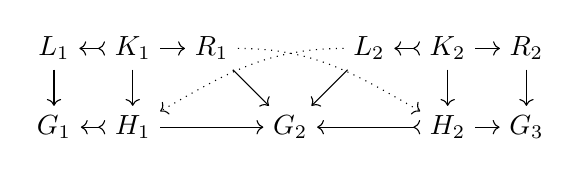
\begin{tikzpicture}
				\node (A)at(0,1){$L_1$};
				\node (B)at(1,1){$K_1$};
				\node (C)at(2,1){$R_1$};
				\node (D)at(4,1){$L_2$};
				\node (E)at(5,1){$K_2$};
				\node(F) at(6,1){$R_2$};
				\node (G)at(0,0){$G_1$};
				\node (H)at(1,0){$H_1$};
				\node (I)at(3,0){$G_2$};
				\node (L)at(5,0){$H_2$};
				\node (M)at(6,0){$G_3$};
				
				\draw[>->](B)--(A);
				\draw[->](B)--(C);
				\draw[>->](E)--(D);
				\draw[->](E)--(F);
				\draw[>->](H)--(G);
				\draw[->](H)--(I);
				\draw[>->](L)--(I);
				\draw[->](L)--(M);
				\draw[->](A)--(G);
				\draw[->](B)--(H);
				\draw[->](C)--(I);
				\draw[->](D)--(I);
				\draw[->](E)--(L);
				\draw[->](F)--(M);
				\draw[dotted, ->](C) to [out=0, in=150](L);
				\draw[dotted, ->](D)to [out=180, in=30](H);
			\end{tikzpicture}
		\end{center}
		\end{definition} 

\pause 
If a system is linear:
\begin{enumerate}
	\item uniqueness of independence pair; \pause 
	\item Local Church-Rosser Theorem: sequentially independent steps can be switched.
\end{enumerate}

\end{frame}

\begin{frame}{Church-Rosser can fail}\justifying

\begin{columns} 
	\begin{column}{.30\textwidth}\centering 	
\xymatrix@C=16pt@R=1pt{
	& 0 \ar@{-}[dd] \ar@{-}[ddddddl] \ar@{-}[ddddddr] &  \\
	&  & \\
	& 1 \ar@{-}[dd] \ar@{-}[ddddl]  \ar@{-}[ddddr]   &  \\
	&  & \\
	& 2 \ar@{.}[d] \ar@{-}[ddl]   \ar@{-}[ddr]     &  \\
	&  \ar@{.}[dl]   \ar@{.}[dr] & \\
	b \ar@{-}[dr] & & c \ar@{-}[dl]\\
	& a } \\
	$\mathcal{M}$ is the class of the identities.	
\end{column}
	
	\begin{column}{.70\textwidth} \centering
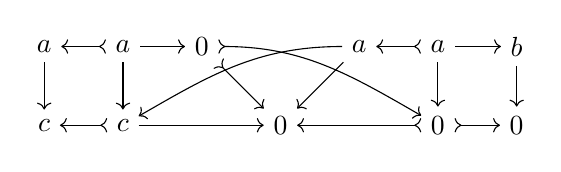
\begin{tikzpicture}
		\node (A)at(0,1){$a$};
		\node (B)at(1,1){$a$};
		\node (C)at(2,1){$0$};
		\node (D)at(4,1){$a$};
		\node (E)at(5,1){$a$};
		\node(F) at(6,1){$b$};
		\node (G)at(0,0){$c$};
		\node (H)at(1,0){$c$};
		\node (I)at(3,0){$0$};
		\node (L)at(5,0){$0$};
		\node (M)at(6,0){$0$};
		
		\draw[>->](B)--(A);
	\draw[->](B)--(C);
	\draw[>->](E)--(D);
	\draw[->](E)--(F);
	\draw[>->](H)--(G);
	\draw[->](H)--(I);
	\draw[>->](L)--(I);
	\draw[>->](L)--(M);
	\draw[->](A)--(G);
	\draw[->](B)--(H);
	\draw[>->](C)--(I);
	\draw[->](D)--(I);
	\draw[->](E)--(L);
	\draw[->](F)--(M);
	\draw[>->](C) to [out=0, in=150](L);
	\draw[->](D)to [out=180, in=30](H);
	\end{tikzpicture}
\\	
Two rewriting steps.
	\end{column}
\end{columns}
 
 \centering
 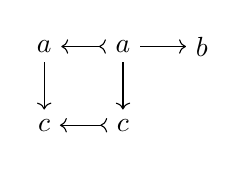
\begin{tikzpicture}
 		\node (A)at(0,1){$a$};
 		\node (B)at(1,1){$a$};
 		\node (C)at(2,1){$b$};
 	
 		\node (G)at(0,0){$c$};
 		\node (H)at(1,0){$c$};
 		
 		\draw[>->](B)--(A);
 		\draw[->](B)--(C);
 	
 		\draw[>->](H)--(G);
 	
 	
 		\draw[->](A)--(G);
 		\draw[->](B)--(H);
 
 	\end{tikzpicture}
\\
No rewriting step.
 
\end{frame}

\begin{frame}{Well switching rewriting systems}\justifying


\begin{definition}
A rewriting system $(\X, R)$ is \emph{well switching} if independence pairs are unique and the Local Church-Rosser Theorem holds (sequentially independent derivation can be switched).
\end{definition}
\pause 
\begin{block}{Remark}
	It is possible to identify a large class of categories on which every left-linear rewriting system enjoys the Local-Church Rosser Theorem holds (\cite{baldan2011adhesivity}).
\end{block}
\pause 
\begin{block}{Example}In the category $\catname{Graph}$, if the rules of a left-linear rewriting system only merge nodes and their left-hand sides contain no isolated nodes, then the system is well-switching.
\end{block}

\end{frame}

\begin{frame}{Results: the Three Steps Lemma}\justifying

\begin{lemma}  Let
	$\dder{D}_0\cdot \dder{D}_1 \cdot \dder{D}_2$ be a three-steps
	derivation in a well-switching rewriting system. 
	\begin{enumerate}\justifying
		\item
		If $\dder{D}_0$ and $\dder{D}_1$ are independent and there is a
		 sequence of switches
		$\dder{D}_0\cdot \dder{D}_1 \cdot \dder{D}_2 \shift{(1,2)}
		\dder{D}_0 \cdot \dder{D}_2' \cdot \dder{D}_1' \shift{(0,1)}
		\dder{D}_2'' \cdot \dder{D}_0' \cdot \dder{D}_1'$ then
		in the last derivation $\dder{D}_0'$ and $\dder{D}_1'$ are independent;
		
		\item
		\label{lem:indep-global-left:2}
		Suppose that $\dder{D}_1$ and $\dder{D}_2$ are independent, and that, in $\dder{D}_0\cdot \dder{D}_1 \cdot \dder{D}_2 \shift{(1,2)}
		\dder{D}_0 \cdot \dder{D}_2' \cdot \dder{D}_1'$, $\dder{D}_0$ and $\dder{D}_2'$ are independent.  If there
		is a switching sequence
		$\dder{D}_0\cdot \dder{D}_1 \cdot \dder{D}_2 \shift{(0,1)}
		\dder{D}_1' \cdot \dder{D}_0' \cdot \dder{D}_2 \shift{(1,2)}
		\dder{D}_1' \cdot \dder{D}_2' \cdot \dder{D}_0''$ then in the last derivation $\dder{D}_1'$ and $\dder{D}_2'$ are independent.
	\end{enumerate}
\end{lemma}
\end{frame}


\begin{frame}{Results: the Three Steps Lemma}\justifying
	
	\begin{lemma}  Let
		$\dder{D}_0\cdot \dder{D}_1 \cdot \dder{D}_2$ be a three-steps
		derivation in a well-switching rewriting system. \pause 
		\begin{enumerate}\justifying
			\item
			If $\dder{D}_0$ and $\dder{D}_1$ are independent and there is a
			sequence of switches
			$\dder{D}_0\cdot \dder{D}_1 \cdot \dder{D}_2 \shift{(1,2)}
			\dder{D}_0 \cdot \dder{D}_2' \cdot \dder{D}_1' \shift{(0,1)}
			\dder{D}_2'' \cdot \dder{D}_0' \cdot \dder{D}_1'$ then
			in the last derivation $\dder{D}_0'$ and $\dder{D}_1'$ are independent; \pause 
			
			\item 
			suppose that $\dder{D}_1$ and $\dder{D}_2$ are independent, and that, in $\dder{D}_0\cdot \dder{D}_1 \cdot \dder{D}_2 \shift{(1,2)}
			\dder{D}_0 \cdot \dder{D}_2' \cdot \dder{D}_1'$, $\dder{D}_0$ and $\dder{D}_2'$ are independent.  If there
			is a switching sequence
			$\dder{D}_0\cdot \dder{D}_1 \cdot \dder{D}_2 \shift{(0,1)}
			\dder{D}_1' \cdot \dder{D}_0' \cdot \dder{D}_2 \shift{(1,2)}
			\dder{D}_1' \cdot \dder{D}_2' \cdot \dder{D}_0''$ then in the last derivation $\dder{D}_1'$ and $\dder{D}_2'$ are independent.
		\end{enumerate}
	\end{lemma}
\end{frame}

\begin{frame}{Results: the Three Steps Lemma}\justifying
Meaning of the previous the previous Lemma: \pause 
\begin{enumerate}
	\item if two derivation steps are independent and we are able to \emph{anticipate} something, then the steps remains independent; \pause 
	\item the independence of two derivation steps can depend on the steps before them, in particular \emph{posticipating} something does not preserves independence.
\end{enumerate}
\pause 

\begin{block}{Remark}
The possibility of losing independence posticipating a derivation is due to left-linearity: it can be proved that in linear systems \emph{independence is global}, i.e. that given two independent contiguous steps, if  at the end of a sequence of switchings they are again contiguous, then they are also still independent (\cite{heindel2009category}).
\end{block}




\end{frame}



\begin{frame}{Results: Canonical Form}\justifying
	
	\begin{theorem}[No need of useless switches]
		Let $\der{D}$ and $\der{D}'$ be derivations If $\der{D} \shifteq[\sigma] \der{D}'$ then there is a switching sequence 
		%\begin{center}
		$\der{D} \shift{\nu_1} \der{D}_1 \shift{\nu_2} \ldots
		\shift{\nu_n} \der{D}'$
		%\end{center}
		consisting only of inversions for $\sigma$ (i.e. permutations $(i, i+1)$ such that $\sigma(i)>\sigma(i+1)$).
	\end{theorem}
\pause 	
\begin{theorem}[Canonical form]
	Let $\der{D}$ and $\der{D}'$ be derivations. If
	$\der{D} \shifteq[\sigma]\der{D}'$ then there is a switching sequence
	\begin{center}
		$\der{D} \shift{\nu_1} \der{D}_1 \shift{\nu_2} \ldots
		\shift{\nu_n} \der{D}'$
	\end{center}
	where for $i \in [1,n]$ we have $\nu_i  = \transp{k}$ with 
	$k = \max \{ j \mid \transp{j} \in \inv{\nu_{i,n}}\}$.
\end{theorem}
\end{frame}


\begin{frame}{Future works}\justifying 
	This work is only the first step in an attempt to construct a concurrent semantics for left-linear DPO rewriting systems.
	
	\smallskip \pause 
	
	In \cite{baldan2017domains} a category of domains, called \emph{weak prime domains} has been proposed as a possible concurrent semantic for systems allowing fusions. 	
	
	\smallskip \pause We plan to build on the results proved in this paper to show that to every left-linear DPO rewriting system it is possible to associate one of these domains, representing ``derivation up to switches''.
\end{frame}

\begin{frame}{\hspace{1pt}}
	\LARGE
	\begin{center}
		Thank you for your attention!
	\end{center}
	
\end{frame}


\section{Bibliography}
\begin{frame}[allowframebreaks]{Bibliography}\justifying 
\printbibliography
\end{frame}

\end{document}